\documentclass[logo,dosguias,magister,propuesta]{tesis-postgrado}
% opciones: logo,dosguias,magister,doctorado,propuesta,txfonts

\keywords{XML; Key Implication}

\begin{document}
\baselineskip 23pt
% ----------------------------------------------------------
% ----------- PARTE INICIAL --------------------------------
\thispagestyle{empty}
% Rellenar con la informacion personal y del trabajo

\titulo{Claves XML: Una Implementaci\'on de Algoritmos de Implicaci\'on y Validaci\'on}

\autor{Emir Fernando Mu\~noz Jim\'enez}
\email{emir@emunoz.org}
\telefono{+569 1234 5678}
\run{12.345.678-9}
\annoingreso{2009}

\fecha{Lunes}{30}{Mayo}{2011}

\profesorguia{Dr.\ Pepito Uno}
\profesorcoguia{Dr.\ Pepito Dos}

\ciudad{Santiago}
\pais{Chile}

\makecubierta

\makecopyright % si es propuesta no se mostrará
% ----------------------------------------------------------
% ----------- PRIMERA PARTE --------------------------------
\frontmatter
% ### Resumen e Indices ####
\include{chapters/gracias}
\include{chapters/dedicatoria}

\resumenCastellano{
La flexibilidad sintáctica, y el complejo anidamiento de los datos en una estructura tipo árbol 
dificulta expresar propiedades deseables de los datos XML, ofreciendo una capacidad limitada para 
expresar semántica. En esta tesis se presenta un estudio de las claves como restricciones de 
integridad sobre documentos XML, implementando algoritmos para los problemas de implicación y 
validación, con el fin de mostrar la factibilidad de usar las capacidades semánticas que éstas 
entregan, y que XML como modelo requiere.
\vspace*{0.5cm}
\KeywordsES{XML; Claves XML; Implicación de claves; Validación de documentos XML; Cover no redundante}
}

\newpage

\resumenIngles{
The syntactic flexibility and complex tree-like nested data make it challenging to express desirable 
properties of XML data, offering a limited capability to express semantic. In this thesis, we present 
a study of keys as integrity constraints on XML documents, implementing algorithms for implication 
and validation problems, with the aim of showing the factibility of using the semantic capabilities 
that keys gives and XML as a model requires.
\vspace*{0.5cm}
\KeywordsEN{XML; XML keys; Key implication; XML document validation; Non-redundant cover}
}

\pagestyle{fancy}
\fancyhead[L]{\slshape \leftmark}
\fancyhead[C]{}
\fancyhead[R]{\thepage}
\tableofcontents        %% Indice general
\listoffigures          %% Indice de figuras
\listoftables           %% Indice de tablas
\listofalgorithms       %% Indice de algoritmos
% ----------------------------------------------------------
% ----------- SEGUNDA PARTE --------------------------------
\mainmatter
% ### Configuración del header ###
\pagestyle{fancy}
\fancyhead[L]{\slshape \leftmark}
\fancyhead[C]{}
\fancyhead[R]{\thepage}
\pagenumbering{arabic}
% ### Capitulos de la tesis ###
\include{chapters/1-intro}
%--------Preliminares
%--------Emir Muñoz Jiménez
%--------13-10-2010

\chapter{Marco Te\'orico}
\label{cap:preliminares}


\section{Documentos XML}


% Figura: \'Arbol XML 1
\begin{figure}[tp]
  \centering
  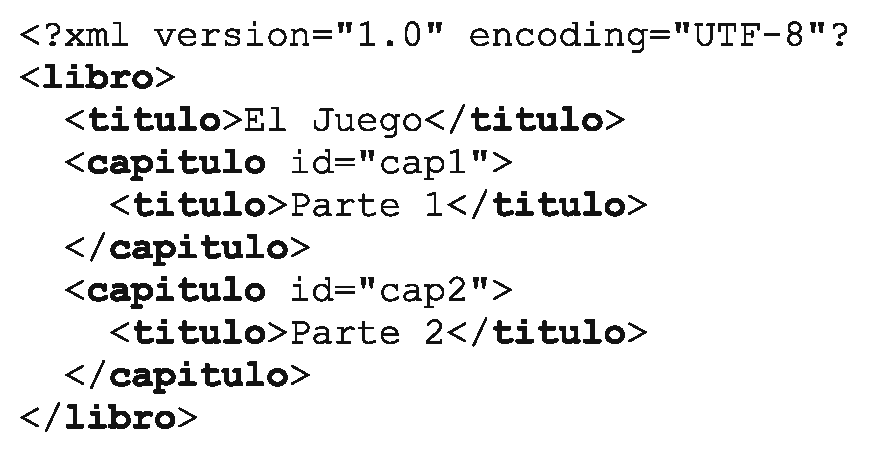
\includegraphics[scale=.5]{images/XML-document-example1}
  \caption{\em Modelo de árbol para un documento XML.}
  \label{fig:xml-tree-exa1}
\end{figure}

\section{El modelo de \'arbol XML}

% ----------------------------------------------------------
% ----------- TERCERA PARTE --------------------------------
% \backmatter %Elimina la numeración
% ### Bibliografía de este documento ###
\bibliographystyle{apa-good}
\bibliography{referencias}
% ----------------------------------------------------------
% ----------- CUARTA PARTE ---------------------------------
\appendix
\addappheadtotoc %agregar Apéndice al índice. Si no tiene apéndices COMENTAR o BORRAR
% \noappendicestocpagenum %quitar número de páginas a los apéndices
% ### ANEXOS ###
%--------Apendice
%--------Emir Muñoz Jiménez
%--------13-10-2010

\chapter{Manual de Usuario}
\label{cap:manual}


\section{Requerimientos}

blablablabla....

\section{Instalaci\'on}

blablablabla....

blablablabla....
 % Manuales de Usuario
\end{document}
%\\end
